\documentclass[tikz,border=12pt]{standalone}
\usepackage[T1]{fontenc}
\usepackage{tgheros}
\usepackage{sfmath}
\usepackage{amsmath}
\usepackage{amssymb}
% % \usepackage{fontawesome5} (Removed for publication-grade academic typography) (Removed for publication-grade academic typography)
\usepackage{tikz}
\usetikzlibrary{arrows.meta,positioning,shapes.geometric,fit,backgrounds,calc}
\usepackage{xcolor}

\renewcommand{\familydefault}{\sfdefault}

% Academic Semantic Palette
\definecolor{harvardcrimson}{HTML}{A51C30}
\definecolor{ethdarkblue}{HTML}{1F407A}
\definecolor{ethblue}{HTML}{215CAF}
\definecolor{ethpetrol}{HTML}{007A87}
\definecolor{ethbronze}{HTML}{B87333}
\definecolor{ethpurple}{HTML}{5B4B8A}
\definecolor{ethslate}{HTML}{475569}
\definecolor{cardbg}{HTML}{F8FAFC}
\definecolor{cardborder}{HTML}{CBD5E1}

\definecolor{badredbg}{HTML}{FEF2F2}
\definecolor{badredborder}{HTML}{F87171}
\definecolor{goodtealbg}{HTML}{ECFDF5}
\definecolor{goodtealborder}{HTML}{34D399}
\definecolor{bluebg}{HTML}{EFF6FF}
\definecolor{blueborder}{HTML}{60A5FA}

\begin{document}
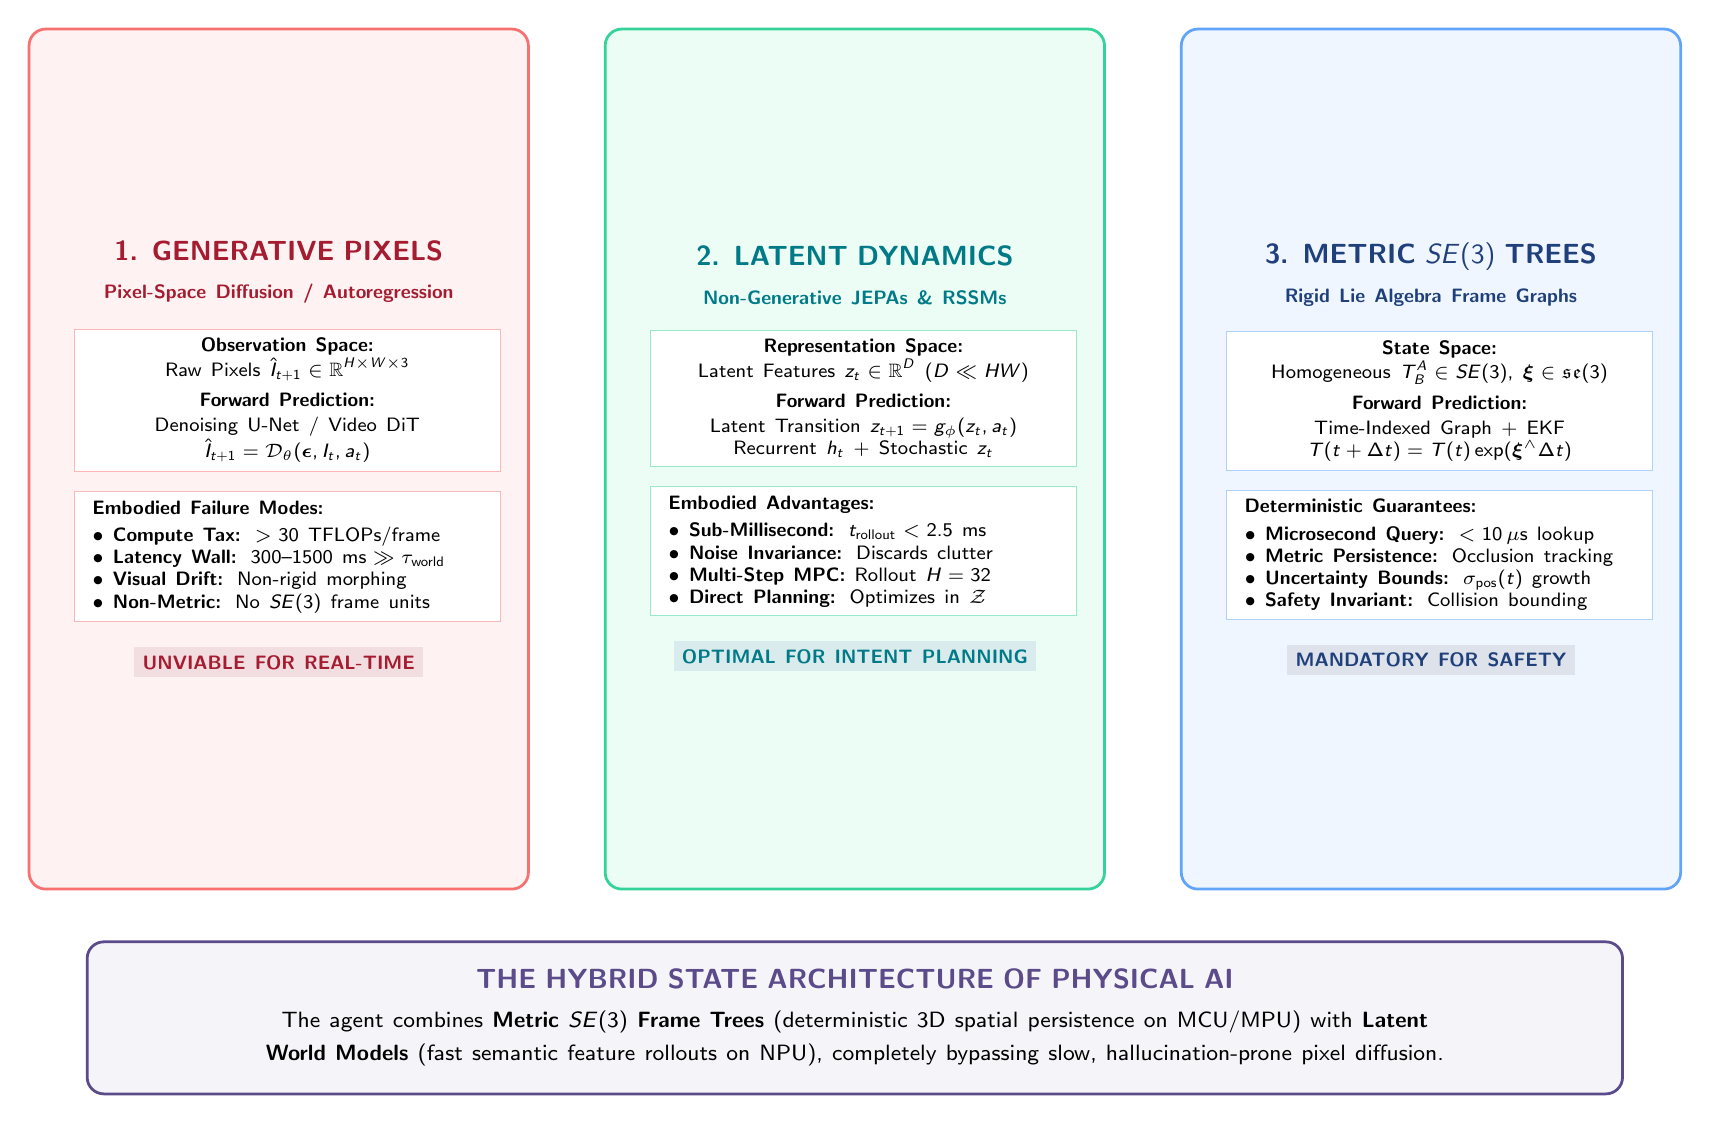
\begin{tikzpicture}[
  font=\sffamily,
  >=Stealth,
  card/.style={
    draw=cardborder,
    fill=white,
    rounded corners=6pt,
    line width=1.0pt,
    inner sep=10pt,
    align=center
  },
  subcard/.style={
    draw=cardborder,
    fill=white,
    rounded corners=4pt,
    line width=0.7pt,
    inner sep=6pt,
    align=center
  }
]

  % Column 1: Generative Pixel Diffusion
  \node[card, draw=badredborder, fill=badredbg, text width=2.22in, minimum height=4.3in, anchor=north west] (col1) at (0, 0) {
    {\bfseries\color{harvardcrimson} 1. GENERATIVE PIXELS}\\[2pt]
    {\scriptsize\bfseries\color{harvardcrimson}Pixel-Space Diffusion / Autoregression}\\[8pt]
    
    \begin{minipage}{2.05in}
      \centering
      \fcolorbox{badredborder!50}{white}{
        \begin{minipage}{1.95in}
          \centering\scriptsize
          \textbf{Observation Space:}\\[1pt]
          Raw Pixels $\hat{I}_{t+1} \in \mathbb{R}^{H \times W \times 3}$\\[3pt]
          \textbf{Forward Prediction:}\\[1pt]
          Denoising U-Net / Video DiT\\
          $\hat{I}_{t+1} = \mathcal{D}_\theta(\boldsymbol{\epsilon}, I_t, a_t)$
        \end{minipage}
      }\\[6pt]
      
      \fcolorbox{badredborder!50}{white}{
        \begin{minipage}{1.95in}
          \raggedright\scriptsize
          \textbf{Embodied Failure Modes:}\\[2pt]
          $\bullet$ \textbf{Compute Tax:} $>30\text{ TFLOPs/frame}$\\
          $\bullet$ \textbf{Latency Wall:} $300\text{--}1500\text{ ms} \gg \tau_{\text{world}}$\\
          $\bullet$ \textbf{Visual Drift:} Non-rigid morphing\\
          $\bullet$ \textbf{Non-Metric:} No $SE(3)$ frame units
        \end{minipage}
      }\\[8pt]
      
      \centering
      \colorbox{harvardcrimson!15}{\scriptsize\bfseries\color{harvardcrimson} UNVIABLE FOR REAL-TIME}
    \end{minipage}
  };

  % Column 2: Latent World Models (JEPA / RSSM)
  \node[card, draw=goodtealborder, fill=goodtealbg, text width=2.22in, minimum height=4.3in, right=0.37in of col1] (col2) {
    {\bfseries\color{ethpetrol} 2. LATENT DYNAMICS}\\[2pt]
    {\scriptsize\bfseries\color{ethpetrol}Non-Generative JEPAs \& RSSMs}\\[8pt]
    
    \begin{minipage}{2.05in}
      \centering
      \fcolorbox{goodtealborder!50}{white}{
        \begin{minipage}{1.95in}
          \centering\scriptsize
          \textbf{Representation Space:}\\[1pt]
          Latent Features $z_t \in \mathbb{R}^D$ ($D \ll HW$)\\[3pt]
          \textbf{Forward Prediction:}\\[1pt]
          Latent Transition $z_{t+1} = g_\phi(z_t, a_t)$\\
          Recurrent $h_t$ + Stochastic $z_t$
        \end{minipage}
      }\\[6pt]
      
      \fcolorbox{goodtealborder!50}{white}{
        \begin{minipage}{1.95in}
          \raggedright\scriptsize
          \textbf{Embodied Advantages:}\\[2pt]
          $\bullet$ \textbf{Sub-Millisecond:} $t_{\text{rollout}} < 2.5\text{ ms}$\\
          $\bullet$ \textbf{Noise Invariance:} Discards clutter\\
          $\bullet$ \textbf{Multi-Step MPC:} Rollout $H=32$\\
          $\bullet$ \textbf{Direct Planning:} Optimizes in $\mathcal{Z}$
        \end{minipage}
      }\\[8pt]
      
      \centering
      \colorbox{ethpetrol!15}{\scriptsize\bfseries\color{ethpetrol} OPTIMAL FOR INTENT PLANNING}
    \end{minipage}
  };

  % Column 3: Metric Spatial Trees (SE(3) + Kalman)
  \node[card, draw=blueborder, fill=bluebg, text width=2.22in, minimum height=4.3in, right=0.37in of col2] (col3) {
    {\bfseries\color{ethdarkblue} 3. METRIC $SE(3)$ TREES}\\[2pt]
    {\scriptsize\bfseries\color{ethdarkblue}Rigid Lie Algebra Frame Graphs}\\[8pt]
    
    \begin{minipage}{2.05in}
      \centering
      \fcolorbox{blueborder!50}{white}{
        \begin{minipage}{1.95in}
          \centering\scriptsize
          \textbf{State Space:}\\[1pt]
          Homogeneous $T_B^A \in SE(3)$, $\boldsymbol{\xi} \in \mathfrak{se}(3)$\\[3pt]
          \textbf{Forward Prediction:}\\[1pt]
          Time-Indexed Graph + EKF\\
          $T(t+\Delta t) = T(t) \exp(\boldsymbol{\xi}^\wedge \Delta t)$
        \end{minipage}
      }\\[6pt]
      
      \fcolorbox{blueborder!50}{white}{
        \begin{minipage}{1.95in}
          \raggedright\scriptsize
          \textbf{Deterministic Guarantees:}\\[2pt]
          $\bullet$ \textbf{Microsecond Query:} $< 10\,\mu\text{s}$ lookup\\
          $\bullet$ \textbf{Metric Persistence:} Occlusion tracking\\
          $\bullet$ \textbf{Uncertainty Bounds:} $\sigma_{\text{pos}}(t)$ growth\\
          $\bullet$ \textbf{Safety Invariant:} Collision bounding
        \end{minipage}
      }\\[8pt]
      
      \centering
      \colorbox{ethdarkblue!15}{\scriptsize\bfseries\color{ethdarkblue} MANDATORY FOR SAFETY}
    \end{minipage}
  };

  % Bottom Synthesis Banner
  \node[card, draw=ethpurple, fill=ethpurple!6, text width=7.4in, below=0.25in of col2.south, anchor=north] (footer) {
    {\bfseries\color{ethpurple} THE HYBRID STATE ARCHITECTURE OF PHYSICAL AI}\\[2pt]
    {\footnotesize The agent combines \textbf{Metric $SE(3)$ Frame Trees} (deterministic 3D spatial persistence on MCU/MPU) with \textbf{Latent World Models} (fast semantic feature rollouts on NPU), completely bypassing slow, hallucination-prone pixel diffusion.}
  };

\end{tikzpicture}
\end{document}
